% ===========================================================================
\section{Cavity design}
% ===========================================================================

\subsection{Constraints set by the magnet and the deposition system}

The cavity design answers to two machines at once. The magnet bore fixes the outer diameter, and the deposition chamber fixes the wall thickness. A Quantum Design Physical Property Measurement System (PPMS) supplies \qty{9}{\tesla} and \qty{2}{\kelvin} with a bore that limits the cavity outer diameter to \qty{26}{\milli\meter}. Subtracting the wall thickness puts the TM$_{010}$ resonance above \qty{10}{\giga\hertz}. That is well above the \qty{4}{\giga\hertz} target of a real haloscope, and the frequency difference must be carried through any comparison with the literature. A larger bore of \qty{40}--\qty{100}{\milli\meter} would allow a lower-frequency cavity, but it costs more capital, more helium, and more waiting for beam time. Designing to PPMS dimensions instead lets a coating be built and tested in weeks, and the same cavity fits the dilution refrigerator at Lawrence Livermore National Laboratory (LLNL). The sputtering and evaporation chambers impose the second limit: no cavity piece may exceed \qty{13}{\milli\meter} in thickness (Fig.~\ref{fig:ClearenceSputter}).

\begin{figure}[htb]
    \centering
    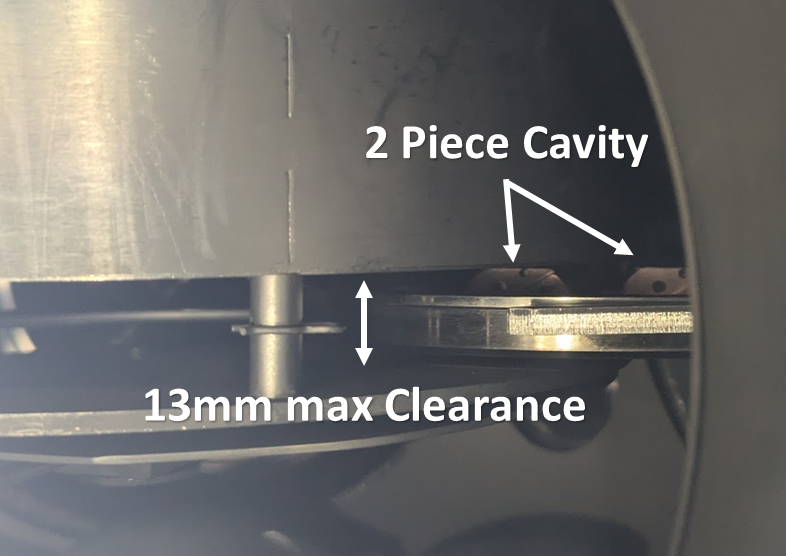
\includegraphics[width=0.7\linewidth]{images/AndreCavity/ClearenceSputter.png}
    \caption{Clearance in the sputtering chamber, which limits any cavity piece to \qty{13}{\milli\meter} thickness.}
    \label{fig:ClearenceSputter}
\end{figure}

Six requirements follow from these constraints and from the physics of the measurement:

\begin{enumerate}
    \item Support an optimization loop that raises $Q$ at \qty{2}{\kelvin} and \qty{9}{\tesla}.
    \item Fit the evaporator and sputtering chamber, so no piece exceeds \qty{13}{\milli\meter} thick.
    \item Fit the magnet bore when assembled, so the outer diameter stays below \qty{26}{\milli\meter}.
    \item Present flat or gently inclined surfaces to line-of-sight deposition sources.
    \item Allow hybrid builds that swap superconducting and normal-conducting walls and endcaps.
    \item Fit inside the \qty{55}{\milli\meter} homogeneous field region of the magnet.
\end{enumerate}

Requirement 5 follows from Braine's measurement on a bulk NbTi cavity~\cite{Braine:2024nzi}. A mode-decomposition analysis showed that the NbTi endcaps became more resistive than copper above \qty{0.3}{\tesla}, while the NbTi walls stayed at low resistance out to \qty{9}{\tesla}. Surfaces perpendicular to the applied field dissipate; surfaces parallel to it do not. A hybrid cavity with copper endcaps and superconducting walls therefore beats a fully superconducting one in field, and the design must permit that swap.

\subsection{Why a hexagonal prism}

Braine's cavity is a cylinder, and a cylinder is the wrong shape for a two-piece cavity that must be coated by line-of-sight sources. Its curved wall sits at \qty{90}{\degree} to the deposition flux along its entire length, and its axial symmetry spreads surface current uniformly along the wall, so any seam sits in full current. Replacing the cylinder with an upright polygon fixes both problems. The idea came from the CAPP REBCO ``orange wedge'' cavity, which similarly exploits the alignment of seams with the current pattern~\cite{ahnSuperconductingCavityHigh2020}.

Finite-element simulation quantifies the seam advantage (Fig.~\ref{fig:GapnoGapCylinderHexagon}). Modelled with \qty{5}{\milli\ohm} walls and a \qty{1}{\ohm} gap, a seamless hexagon has $\sim$9\% lower $Q$ than a seamless cylinder, purely from geometry. Introducing two resistive seams on the wall reverses the ranking: the cylinder loses $\sim$27\% of its $Q$, the hexagon $\sim$1\%. A hexagon concentrates surface current at the centre of each face and starves the corners, so a seam placed on a corner carries almost no current. That single result justifies the geometry for every cavity in this work.

\begin{figure}[htb]
    \centering
    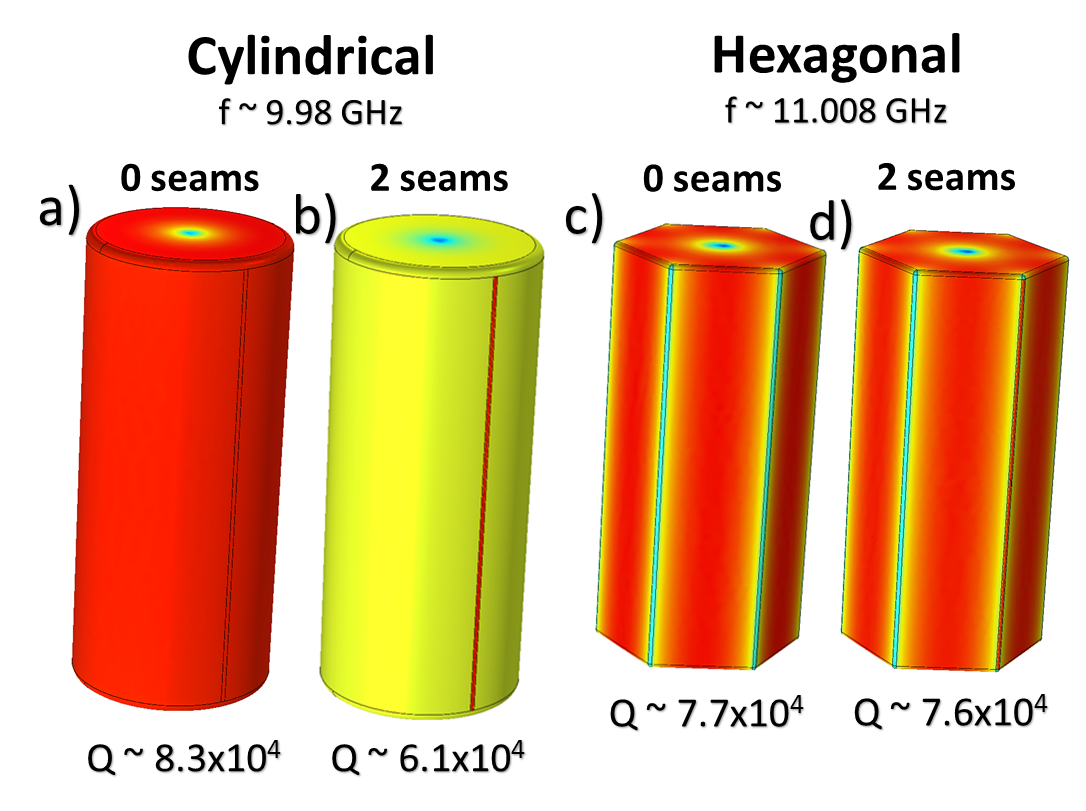
\includegraphics[width=0.8\linewidth]{images/AndreCavity/GapnoGapCylinderHexagon.png}
    \caption[COMSOL simulation of cylinder and hexagon cavities with and without a resistive seam.]{COMSOL simulation of frequency and quality factor for cylinder (a, b) and hexagon (c, d) geometries. The colour scale shows surface current, red maximum and green minimum. Input surface resistance is \qty{5}{\milli\ohm} for the walls and \qty{1}{\ohm} for the gap. Comparing (b) with (d) shows that the hexagon loses far less to a seam at its edge.}
    \label{fig:GapnoGapCylinderHexagon}
\end{figure}

The hexagon also helps deposition. A cylindrical wall is normal to the source at \qty{90}{\degree}, whereas a hexagonal wall cut at the polygon edge presents at most \qty{60}{\degree} (Fig.~\ref{fig:Angle8piece}). Thermal evaporation is line-of-sight, so that \qty{30}{\degree} difference decides whether the long edge of the cavity receives film at all.

\begin{figure}[htb]
    \centering
    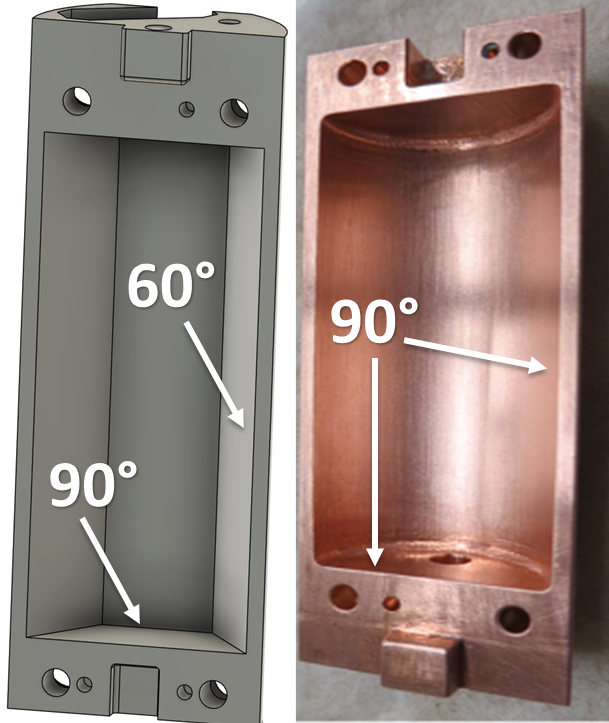
\includegraphics[width=0.5\linewidth]{images/AndreCavity/Angle8piece.png}
    \caption[Hexagonal versus cylindrical inner-surface angles relative to the deposition source.]{Hexagonal and cylindrical two-piece designs showing the angle of the inner surface normal to the incoming vapour flux. Zero degrees is a flat sample; \qty{90}{\degree} is the steepest angle a line-of-sight source can coat.}
    \label{fig:Angle8piece}
\end{figure}

\subsection{Returning to a cylinder}

The hexagon wins on seams and on deposition angle, and it loses on polishing. Its inner corners are acute, and reaching them by hand requires wrapping abrasive around an eraser and working one face at a time. A cylinder has no corners, so hand polishing and electropolishing both reach every part of the surface with uniform pressure and uniform current density. Copper surface quality turned out to dominate the measured $Q$ of every cavity in this work, which reorders the trade-off: a seam penalty of \qty{27}{\percent} is smaller than the penalty already being paid for an imperfectly polished surface. The final two cavities therefore return to Braine's cylindrical geometry~\cite{Braine:2024nzi} with an improved surface preparation, so that the coating is compared against a copper baseline that is as good as the copper can be.

\subsection{Mode selection}

Axion conversion scales with $\mathbf{E}_\text{AC}\cdot\mathbf{B}_0$, so the cavity mode must put its electric field along the solenoid axis. For a vertical cylinder or prism in a solenoid, TM$_{010}$ does exactly that. It is also the fundamental, so it fills the cavity volume without nodal planes that would waste interaction region. Every $Q$ reported here is the TM$_{010}$ value with the cavity axis parallel to the applied field, which reproduces the field geometry of an operating haloscope.
